\documentclass[aspectratio=169,10pt]{beamer}
\usepackage{tikz}
\usepackage[scaled=.92]{helvet}
\renewcommand{\familydefault}{\sfdefault}
\usetikzlibrary{positioning,arrows.meta,calc}
\definecolor{bg}{HTML}{071014}
\definecolor{panel}{HTML}{101D22}
\definecolor{active}{HTML}{16262C}
\definecolor{line}{HTML}{2A3D43}
\definecolor{text}{HTML}{E8F0F1}
\definecolor{muted}{HTML}{8AA0A5}
\definecolor{green}{HTML}{69D69A}
\definecolor{mint}{HTML}{A4F0C3}
\definecolor{amber}{HTML}{E8B85E}
\definecolor{red}{HTML}{EC746D}
\definecolor{blue}{HTML}{78B8DB}
\setbeamercolor{background canvas}{bg=bg}
\setbeamercolor{normal text}{fg=text,bg=bg}
\setbeamercolor{frametitle}{fg=text,bg=bg}
\setbeamercolor{block title}{fg=text,bg=active}
\setbeamercolor{block body}{fg=text,bg=panel}
\setbeamertemplate{blocks}[rounded][shadow=false]
\setbeamertemplate{navigation symbols}{}
\setbeamersize{text margin left=7mm,text margin right=7mm}
\setbeamerfont{frametitle}{size=\LARGE,series=\bfseries}
\setbeamerfont{block title}{series=\bfseries}
\setbeamertemplate{itemize item}{\color{mint}$\blacktriangleright$}
\setbeamertemplate{footline}{\hfill{\color{muted}\scriptsize HELIOS -- ONE OPERATIONAL WORLD \quad \insertframenumber/\inserttotalframenumber\hspace{6mm}\vspace{3mm}}}
\newcommand{\status}[2]{\textcolor{#1}{\scriptsize\bfseries #2}}
\newcommand{\tagcurrent}{\status{green}{CURRENT}}
\newcommand{\tagdev}{\status{amber}{IN DEVELOPMENT}}
\newcommand{\tagplanned}{\status{blue}{PLANNED}}
\begin{document}

\begin{frame}[plain]
\begin{tikzpicture}[remember picture,overlay]
  \fill[blue,opacity=.05] (13,2.5) circle (3.6);
  \draw[mint,opacity=.18,line width=18pt] (13,2.5) circle (2.3);
  \draw[blue,opacity=.24,line width=4pt] (13,2.5) circle (3.2);
  \draw[green,opacity=.38,line width=1.1pt] (9.8,.5)--(15.8,5.7);
  \fill[green,opacity=.75] (12.1,3.25) circle (.10);
  \fill[amber,opacity=.85] (13.5,2.05) circle (.12);
  \fill[blue,opacity=.85] (14.6,3.45) circle (.09);
\end{tikzpicture}
\vspace{9mm}
{\color{mint}\Large\bfseries HELIOS}\par
\vfill
{\color{text}\fontsize{31}{35}\selectfont\bfseries One Operational World}\par\vspace{3mm}
{\color{text}\Large A concise guide to AI-assisted and autonomous Site operations}\par\vspace{8mm}
{\color{green}\large AI + AUTONOMY + PEOPLE + ROBOTICS}\par
\vfill
{\color{muted}\small Proposed user experience based on the currently understood Helios environment}\hfill{\color{muted}\small Version 0.1 -- August 2026}
\end{frame}

\begin{frame}{What Helios actually is}
{\large One governed environment for understanding conditions, coordinating response, supervising autonomy, and proving outcomes.}\vspace{3mm}
\begin{columns}[T]
\column{.32\textwidth}
\begin{block}{Operational world}
\small Digital Twin, Sites, zones, routes, sensors, robotic assets, human teams, evidence, and readiness.
\end{block}
\column{.32\textwidth}
\begin{block}{Governed action}
\small Attention, Incidents, Missions, resources, Commands, intervention, observed effects, and Records.
\end{block}
\column{.32\textwidth}
\begin{block}{Cortex intelligence}
\small Assessment, recommendations, policy-bounded intent, memory, learning, and Agent coordination.
\end{block}
\end{columns}
\vspace{3mm}
\begin{block}{The principle}
\centering Existing systems retain the authority they should own. Helios connects them into one operational and autonomy layer.
\end{block}
\vfill
\centering \tagcurrent\ Foundations \quad \tagdev\ Mission + Command integration \quad \tagplanned\ Autonomy + coordination
\end{frame}

\begin{frame}{One Site. One event. One shared context.}
\begin{columns}[T]
\column{.43\textwidth}
\begin{block}{02:14 -- west restricted perimeter}
\small
\begin{itemize}
  \item Fixed visible camera reports motion.
  \item Thermal source is consistent with a person.
  \item No matching access event is present.
  \item Visual identity remains unknown.
  \item One aerial asset is available.
  \item A ground robot is staged nearby.
\end{itemize}
\end{block}
\begin{block}{Attention created}
\small Helios shows consequence, uncertainty, source freshness, nearby capabilities, route restrictions, reserve coverage, and current authority.
\end{block}
\column{.54\textwidth}
\centering{\scriptsize NORTH RIVER ENERGY CAMPUS -- FICTIONAL ILLUSTRATION}\par\vspace{2mm}
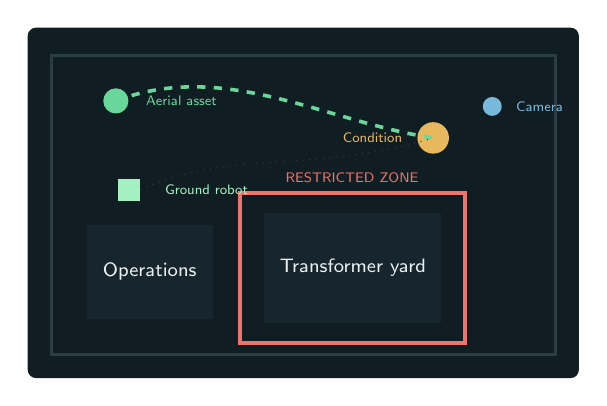
\begin{tikzpicture}[x=1cm,y=1cm]
  \fill[panel,rounded corners=3pt] (0,0) rectangle (7,4.45);
  \draw[line,line width=1pt] (.3,.3) rectangle (6.7,4.1);
  \fill[active] (.75,.75) rectangle (2.35,1.95);
  \node[text=text,font=\scriptsize] at (1.55,1.35){Operations};
  \fill[active] (3,.7) rectangle (5.25,2.1);
  \node[text=text,font=\scriptsize] at (4.13,1.4){Transformer yard};
  \draw[red,line width=1.5pt] (2.7,.45) rectangle (5.55,2.35);
  \node[red,font=\tiny] at (4.12,2.55){RESTRICTED ZONE};
  \fill[blue] (5.9,3.45) circle (.12);
  \node[blue,font=\tiny,anchor=west] at (6.08,3.45){Camera};
  \fill[amber] (5.15,3.05) circle (.20);
  \node[amber,font=\tiny,anchor=east] at (4.88,3.05){Condition};
  \fill[green] (1.12,3.52) circle (.16);
  \node[green,font=\tiny,anchor=west] at (1.38,3.52){Aerial asset};
  \draw[green,dashed,line width=1.3pt] (1.12,3.52) .. controls (2.5,4.05) and (3.8,3.25) .. (5.15,3.05);
  \fill[mint] (1.15,2.25) rectangle (1.43,2.53);
  \node[mint,font=\tiny,anchor=west] at (1.62,2.39){Ground robot};
  \draw[line,dotted] (1.43,2.39) .. controls (2.5,2.9) and (3.7,2.6) .. (5.15,3.05);
\end{tikzpicture}
\end{columns}
\vfill
{\color{muted}\small Selection is inspection. No map click, camera movement, or Cortex statement creates a physical effect.}
\end{frame}

\begin{frame}{The same event at increasing authority levels}
\begin{columns}[T]
\column{.32\textwidth}
\begin{block}{PHASE 1 -- OPERATOR DIRECTED}
\small Helios presents evidence, world context, qualified resources, route, readiness, and consequence. The operator creates and launches the Mission.\vspace{2mm}\par
{\color{green}\bfseries Human role: direct.}
\end{block}
\column{.32\textwidth}
\begin{block}{PHASE 2 -- CORTEX ASSISTED}
\small Cortex correlates evidence, explains uncertainty, compares options, and recommends an aerial Mission. The operator accepts, modifies, rejects, or asks why.\vspace{2mm}\par
{\color{amber}\bfseries Human role: decide.}
\end{block}
\column{.32\textwidth}
\begin{block}{PHASE 3 -- POLICY AUTONOMY}
\small Evidence and policy qualify. Cortex initiates the approved observation Mission through normal readiness, resource, and Command admission.\vspace{2mm}\par
{\color{blue}\bfseries Human role: supervise.}
\end{block}
\end{columns}
\vspace{4mm}
\begin{block}{PHASE 4 -- MULTI-AGENT COORDINATION}
\centering Site, Asset, Mission, and Operations Agents request and broker capabilities. Humans govern priorities, exceptions, policy, and consequence.
\end{block}
\end{frame}

\begin{frame}{Conceptual operational view}
{\color{blue}\scriptsize\bfseries CONCEPTUAL OPERATIONAL VIEW -- PROPOSED USER EXPERIENCE}\vspace{2mm}
\begin{columns}[T]
\column{.23\textwidth}
\begin{block}{ATTENTION}
\scriptsize
{\color{amber}\bfseries WEST PERIMETER}\par Multi-source event\par Age 00:21\par Policy-initiated Mission\par\vspace{2mm}
{\color{red}\bfseries NORTH COVERAGE}\par Reserve reduced 8\%\par\vspace{2mm}
{\color{muted}Human judgment not yet required}
\end{block}
\column{.49\textwidth}
\begin{block}{TACTICAL WORLD}
\centering
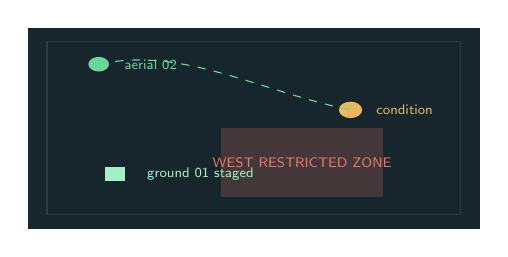
\begin{tikzpicture}[x=.82cm,y=.58cm]
  \fill[active] (0,0) rectangle (7,4.4);
  \draw[line] (.3,.3) rectangle (6.7,4.1);
  \fill[red,opacity=.22] (3,.7) rectangle (5.5,2.2);
  \node[red,font=\tiny] at (4.25,1.45){WEST RESTRICTED ZONE};
  \fill[amber] (5,2.6) circle (.18);
  \node[amber,font=\tiny,anchor=west] at (5.25,2.6){condition};
  \fill[green] (1.1,3.6) circle (.16);
  \node[green,font=\tiny,anchor=west] at (1.35,3.6){aerial 02};
  \draw[green,dashed] (1.1,3.6) .. controls (2.4,4) and (3.6,3) .. (5,2.6);
  \fill[mint] (1.2,1.05) rectangle (1.5,1.35);
  \node[mint,font=\tiny,anchor=west] at (1.7,1.2){ground 01 staged};
\end{tikzpicture}
\par\scriptsize Mission: Investigate west perimeter
\end{block}
\column{.25\textwidth}
\begin{block}{CORTEX}
\scriptsize
Assessment\par Person-like thermal source. Visual confirmation incomplete.\vspace{2mm}\par
Policy\par Restricted Perimeter Observation v4.\vspace{2mm}\par
Why Helios acted\par Two current sources, after-hours zone, route valid, reserve preserved.
\end{block}
\end{columns}
\vspace{2mm}
\begin{block}{MISSION AND RECEIPTS}
\scriptsize Tasks: overhead view $\rightarrow$ track $\rightarrow$ inspect blind area $\rightarrow$ preserve evidence \hfill HOLD \quad REDIRECT \quad RETURN \quad ABORT\par\vspace{1mm}
Authorized {\color{green}\bfseries YES} \quad Delivered {\color{green}\bfseries YES} \quad Asset accepted {\color{green}\bfseries YES} \quad Effect observation {\color{amber}\bfseries PENDING}
\end{block}
\end{frame}

\begin{frame}{The Digital Twin is the operational world}
\begin{columns}[T]
\column{.46\textwidth}
\begin{block}{More than a 3D model}
\small
\begin{itemize}
  \item Source geometry, frames, calibration, and uncertainty.
  \item Buildings, zones, routes, POIs, docks, and recovery.
  \item Cameras, sensors, coverage, and freshness.
  \item Asset deployments, capability, and readiness.
  \item Missions, policy, evidence, and revision.
\end{itemize}
\end{block}
\begin{block}{Cortex uses structured context}
\small Location, reachability, coverage, restrictions, resource qualification, route consequence, and evidence relationships.
\end{block}
\column{.51\textwidth}
\begin{block}{One accountable Mission picture}
\centering
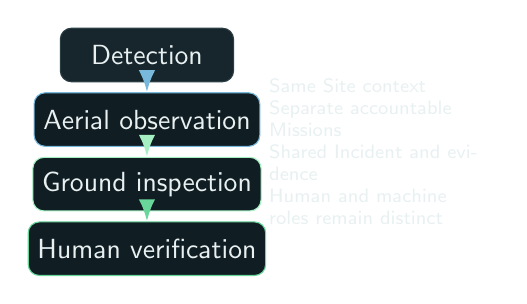
\begin{tikzpicture}[x=.82cm,y=.82cm]
  \node[draw=line,fill=active,text=text,rounded corners,minimum width=2.2cm,minimum height=.68cm] (d) at (1.8,4){Detection};
  \node[draw=blue,fill=panel,text=text,rounded corners,minimum width=2.2cm,minimum height=.68cm] (a) at (1.8,3){Aerial observation};
  \node[draw=mint,fill=panel,text=text,rounded corners,minimum width=2.2cm,minimum height=.68cm] (g) at (1.8,2){Ground inspection};
  \node[draw=green,fill=panel,text=text,rounded corners,minimum width=2.2cm,minimum height=.68cm] (h) at (1.8,1){Human verification};
  \draw[-{Latex},blue,line width=1.1pt] (d)--(a);
  \draw[-{Latex},mint,line width=1.1pt] (a)--(g);
  \draw[-{Latex},green,line width=1.1pt] (g)--(h);
  \node[text=text,font=\scriptsize,align=left,text width=2.8cm] at (5.4,2.5){Same Site context\par Separate accountable Missions\par Shared Incident and evidence\par Human and machine roles remain distinct};
\end{tikzpicture}
\end{block}
\begin{block}{Trust is visible}
\centering\scriptsize Authorized $\rightarrow$ Delivered $\rightarrow$ Accepted $\rightarrow$ Observed $\rightarrow$ Outcome known
\end{block}
\end{columns}
\end{frame}

\begin{frame}{Cortex manages complexity. Attention protects focus.}
\begin{columns}[T]
\column{.48\textwidth}
\begin{block}{ATTENTION answers one question}
\Large What actually needs me now?\vspace{3mm}\par
\small New uncertainty, autonomous activity, degraded communications, resource conflict, unknown Command result, stale evidence, policy exception, or decision due.
\end{block}
\begin{block}{Major Cortex roles}
\small Site Agent \quad Asset Agent \quad Mission Agent \quad Operations Agent\par\vspace{2mm}
{\color{muted}Specific accountable roles under one user-facing Cortex identity.}
\end{block}
\column{.49\textwidth}
\begin{block}{OPERATIONAL EXERCISES}
\small The same world, Missions, assets, Cortex, Attention, controls, and Records can be exercised under unmistakable simulation authority.\vspace{2mm}
\begin{itemize}
  \item Shift and Mission practice.
  \item Communications and sensor degradation.
  \item Autonomous-policy evaluation.
  \item Operator intervention and After-Action Review.
\end{itemize}
\end{block}
\begin{block}{Learning remains governed}
\small Evidence $\rightarrow$ candidate $\rightarrow$ simulation or replay $\rightarrow$ review $\rightarrow$ approved version $\rightarrow$ monitoring and rollback.
\end{block}
\end{columns}
\end{frame}

\begin{frame}{From one Site to the enterprise}
\centering
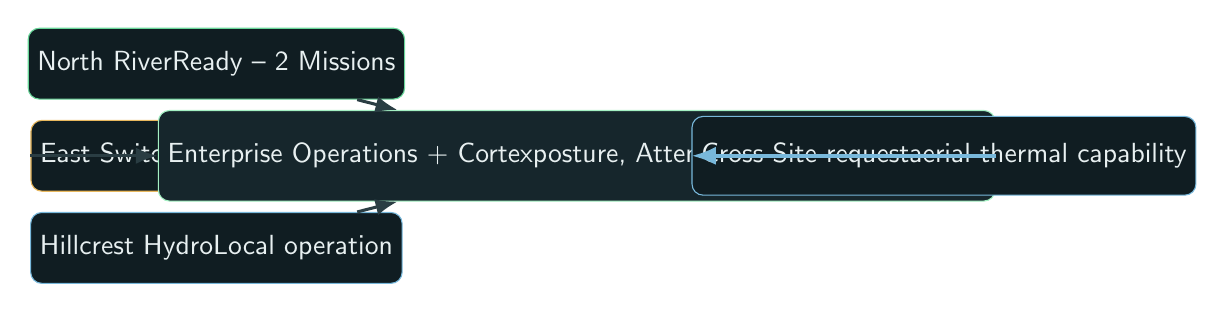
\begin{tikzpicture}[x=.88cm,y=.78cm]
  \node[draw=green,fill=panel,text=text,rounded corners,minimum width=2.7cm,minimum height=.9cm,align=center] (n) at (1.8,3.6){North River\par Ready -- 2 Missions};
  \node[draw=amber,fill=panel,text=text,rounded corners,minimum width=2.7cm,minimum height=.9cm,align=center] (e) at (1.8,2.1){East Switching\par Support needed};
  \node[draw=blue,fill=panel,text=text,rounded corners,minimum width=2.7cm,minimum height=.9cm,align=center] (h) at (1.8,.6){Hillcrest Hydro\par Local operation};
  \node[draw=mint,fill=active,text=text,rounded corners,minimum width=3.8cm,minimum height=1.15cm,align=center] (o) at (7,2.1){Enterprise Operations + Cortex\par posture, Attention, policy, coordination};
  \node[draw=blue,fill=panel,text=text,rounded corners,minimum width=3.1cm,minimum height=1cm,align=center] (r) at (12.3,2.1){Cross-Site request\par aerial thermal capability};
  \draw[-{Latex},line,line width=1.1pt] (n)--(o);
  \draw[-{Latex},line,line width=1.1pt] (e)--(o);
  \draw[-{Latex},line,line width=1.1pt] (h)--(o);
  \draw[-{Latex},blue,line width=1.3pt] (o)--(r);
\end{tikzpicture}
\vspace{2mm}
\begin{block}{The payoff}
\centering{\Large\bfseries Your systems. Your Sites. One coherent operating experience.}\par\vspace{1mm}
{\small See the operation. Coordinate the response. Prove the outcome.}
\end{block}
\vfill
\centering \tagcurrent\ Foundations \quad \tagdev\ Canonical integration \quad \tagplanned\ Autonomy, resilient Site cells, and coordination
\end{frame}

\end{document}
